\chapter{Literature Review}\label{lit}
This chapter will investigate the relevant literature on sperm analysis techniques. Mainly there are two parts, comparing traditional computer vision solutions with deep learning approaches and object tracking. The advantages and limitations of each solution will be discussed in this chapter, followed by the various object-tracking solutions. 
\newpage
\section{Traditional Approach}
Traditional computer vision approaches for sperm analysis rely on image processing techniques such as edge detection, thresholding, segmentation, clustering, etc., to extract sperm cells from the background and track their trajectories. The traditional methods usually set predefined physical characteristics for the sperms, such as the color and shape of the head or tails, and they are used to separate the sperms from the background. For example, a sperm tracking system was created by applying a series of Gaussian filters to increase the contrast of the images and applying the Otsu thresholding method to detect the sperms from the background. \cite{trad1} In another study, the Hough transform was used to locate the sperm head, and ellipse detection was followed using five parameters. \cite{trad2} In contrast, Nafisi et al. detected the tails instead, using their size and elongation characteristics to assume the size and position of the sperm heads. \cite{trad3} Lastly, Chang et al. used k-means clustering to detect sperm heads and their tails from the background. \cite{trad4} 

Although these approaches can be run in a relatively computationally limited environment, these methods have several drawbacks that limit their performance and applicability. First, they depend highly on image quality and require a good contrast between the sperms and the background. They may fail to detect sperm cells that are blurry. Second, they are sensitive to noise and occlusion, which may cause false positives or false negatives in detection and tracking. Third, they often require manual tuning of parameters and thresholds, which may vary depending on the sample type and condition. Fourth, they have low flexibility in dealing with different types of sperm samples, such as those with abnormal morphology or motility patterns. Fifth, they have relatively low computational efficiency, involving multiple image processing and feature extraction steps.
\section{Deep Learning Approach}
Deep learning approaches for sperm analysis use neural networks to learn features from raw images and perform tasks such as detection, tracking, classification, etc. Deep neural networks can automatically learn from data without requiring manual feature engineering or parameter tuning once the setting is finished from the early stages of development. They also have higher flexibility and robustness to deal with different types of sperm samples and image quality if trained with various training examples with different conditions. Usually, in sperm detection tasks, convolutional neural networks (CNN) are used to detect sperms. For example, Riordon et al. fine-tuned VGG16, a popular CNN model initially trained on the ImageNet dataset, to classify the sperm head from the images. \cite{deep1} 
\subsection{Multi-Object Detection}
Although classifying individual sperm cells in a small image subsection is relatively easier, detecting multiple sperm cells from an image needs a new set of architectures. While the classification tasks only require one classification output, the detection models require multiple sets of 5 outputs, classification, x-coordinate, y-coordinate, width, and height of each detection. In the early stages of multi-object detection, a technique called 'Sliding Windows' was used. As the name suggests, the detection mask with a predefined width and height moves pixel-by-pixel, sometimes multiple pixels at once, to predict every region for the presence of the sperm cells. Then, the detection results are extracted from the regions with high confidence scores. Semanet et al. successfully adapted this technique to convolutional deep learning models at the ImageNet Large Scale Visual Recognition Challenge 2013 (ILSVRC2013). \cite{deep2} 

Although this technique has shown notable results in the competition, it still has limitations, such as long processing time per image, redundant detection generation, small or occluded images undetected, etc. Such limitations gave rise to the new groundbreaking architecture in object detection, You-Only-Look-Once (YOLO). \cite{deep3} As the name suggests, YOLO is a real-time object detection system that predicts the bounding boxes in only one evaluation. YOLO divides the image into a grid and predicts each grid's bounding boxes, confidence scores, and class probabilities. \cite{deep4} Then, the results from each grid are evaluated according to the algorithm of YOLO output layers. YOLO model has been very efficient and fast, with up to 45 frames per second, whereas the older object detection models could handle only up to 20 frames per second. \cite{deep3} 

Since its introduction in 2016, multiple versions of YOLO have been released, each improving the accuracy and speed of the model. Many researchers have taken success in utilizing various YOLO models for sperm detection. Sato et al. used YOLOv3 for morphology assessment and tracking model. \cite{deep5} Dobrovolny et al. used YOLOv5 for superior performance in both accuracy and speed. \cite{deep6} YOLOv5 also has three output heads, where the model can simultaneously handle tiny, medium, and large objects. \cite{deep6} Zhu et al. have proposed their version of YOLOv5 by using a depthwise, separable convolution structure to replace the partial convolution of the backbone network, which reduces the number of parameters and increases precision. \cite{deep7}
\newpage
Recently, a new version of YOLO architecture has been released. The new state-of-the-art (SOTA) model, YOLOv8, can now handle more difficult tasks with improved speed, size, and accuracy. \cite{deep8} According to the performance benchmarks conducted by Stereolabs, the accuracy of the eighth version, especially for the smaller models, has increased by around 20\%, and the detection speed has increased by 5 to 10\%. \cite{deep9} 

\begin{figure}[h]
\centering
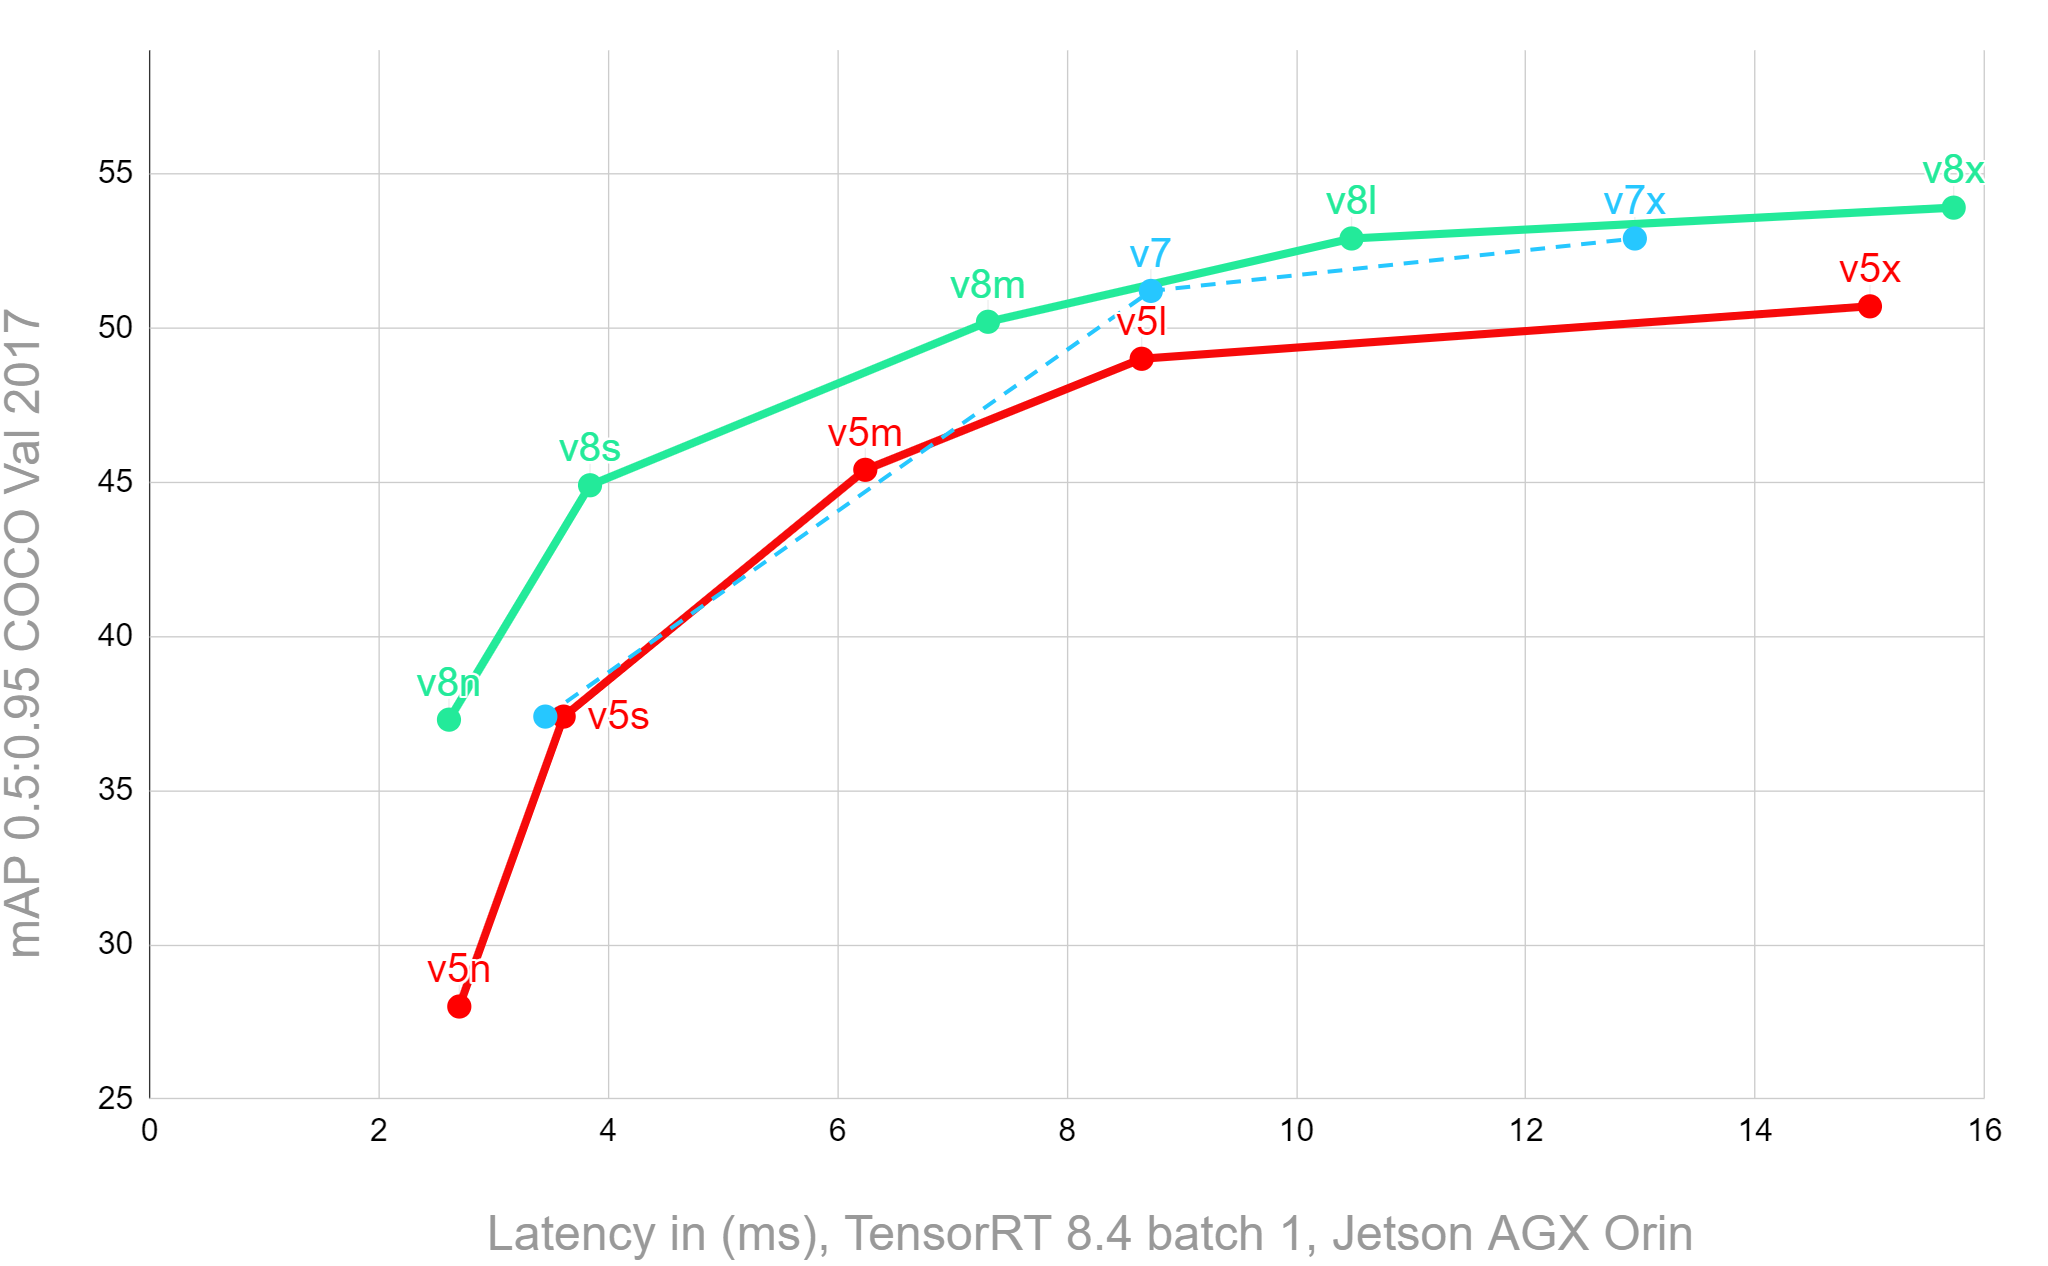
\includegraphics[width=10cm]{Images/YOLO Comparison Chart.png}
\caption{YOLO Comparison Plot \cite{deep9}}
\label{yolocomp}
\end{figure}

Although many researchers have developed and utilized many deep learning models for sperm detection, deep learning still has some drawbacks. Firstly, deep learning models require a lot of data and labeling labor to produce reliable detection results, which are often very expensive. Secondly, even the lightest models require computational resources, such as GPU support and large memory. However, deep learning's advantages make it a better choice for sperm detection. Deep learning models can learn complex and nonlinear features from the data. From the learning, the models can detect the sperm cells flexibly, detecting partially occluded sperms and sperms out of focus from the camera. Therefore, deep learning is still advantageous over traditional approaches.
\newpage
\section{Object Tracking}
Object tracking is a fundamental task in computer vision to locate and identify objects of interest in a video sequence. One main challenge is handling multiple objects simultaneously, especially when they have similar shapes and colors, undergo occlusion, and move unpredictably. Multiple object tracking (MOT) can be formulated as a data association problem, where the goal is to assign identification numbers to objects and build the movement tracks. There are two main categories of object tracking methods: online and offline. Online methods process the detections sequentially and update the tracks in each frame, while offline methods collect all the detections in a batch and optimize the tracks globally. As this project aims to build a real-time detection model, only the online models will be discussed further in this paper.

One of the most well-known online tracking models is Simple-Online-and-Realtime-Tracking (SORT) model built by Bewley et al. \cite{SORT} SORT utilized the Kalman filter to associate objects from different timesteps in sequential frames. The advantage of the Kalman filter in object tracking tasks is that it can predict the current position of an object based on the movement of the same object in previous frames. Moreover, due to its recursive nature, the Kalman filter does not take much space in memory and has a faster execution period, which makes it a favorable choice for real-time tracking tasks. Wojke et al. introduced deep learning techniques to the SORT algorithm, enhancing the original motion model with deep learning components that take account of the visual features of the detections to make better tracking. \cite{DeepSORT}

From many previous pieces of research about sperm tracking, the Kalman filter paired with the Hungarian assignment algorithm works well. From the works of Jati at el., the Kalman filter paired up with the Hungarian assignment algorithm worked well even in low frame rate videos. \cite{KalmanHungarian}